\documentclass[conference]{IEEEtran}
\IEEEoverridecommandlockouts
% Based on the IEEE conference template supplied for WINCOM.

\usepackage{cite}
\usepackage{amsmath,amssymb,amsfonts}
\usepackage{graphicx}
\usepackage{textcomp}
\usepackage{xcolor}
\usepackage{booktabs}
\usepackage{array}
\usepackage{url}
\usepackage{float}
\usepackage{placeins}
\usepackage{tikz}
\usetikzlibrary{arrows.meta,positioning,shapes.geometric,fit}

% Leave tolerance for submission checkers that estimate the gutter from glyph bounds.
\setlength{\columnsep}{0.22in}

% Keep top-of-column figures close to the following text in the two-column layout.
\setlength{\textfloatsep}{8pt plus 1pt minus 2pt}
\setlength{\floatsep}{8pt plus 1pt minus 2pt}

\definecolor{systemblue}{RGB}{41,98,151}
\definecolor{systemgreen}{RGB}{45,126,96}
\definecolor{systemorange}{RGB}{190,104,45}
\definecolor{systempurple}{RGB}{112,76,154}
\definecolor{lightgray}{RGB}{244,246,248}

\begin{document}

\title{\huge A Human-Centered Architecture for Instrumented Virtual Reality Training with Digital Twin Connectivity}

\author{
\IEEEauthorblockN{Saad Joual}
\IEEEauthorblockA{
\textit{FABLAB, HESTIM Casablanca}\\
\textit{ENSAM, Hassan II University of Casablanca}\\
Casablanca, Morocco\\
Saadjawal2003@gmail.com}
\and
\IEEEauthorblockN{Sridath Tula}
\IEEEauthorblockA{
\textit{Centre de Recherche en Ing\'enierie et Management (CERIM)}\\
\textit{HESTIM Engineering \& Business School}\\
Casablanca, Morocco\\
s.tula@hestim.ma}
}

\maketitle

\begin{abstract}
Virtual reality can support industrial training, but a realistic scene alone does not define task order, action validity, or measurable evidence. This paper presents an instrumented platform for a labeling workstation. Implemented in Unity 6 for Meta Quest 3, it represents the task as configurable states coupled to guidance, rule-based validators, and state-level telemetry. A separate read-only ESP32-FastAPI-Unity path demonstrates optional factory supervision without controlling equipment or gating training. Technical evaluation combined requirement-level functional checks with 36 retained session records from 12 students. The logger captured 131 invalid interactions in 31 sessions. Twenty-nine records reconciled total and state durations within approximately 1~ms; seven residuals exposed the absence of explicit session-boundary timestamps. The evaluation concerns architectural behavior rather than training effectiveness; no learning-effect or condition-comparison claim is made. The contribution is an event-driven architecture for inspectable procedural control, recoverable invalid actions, state-level evidence, and decoupled physical-data supervision.
\end{abstract}

\begin{IEEEkeywords}
virtual reality, smart factory, procedural training, digital twin, state machine, interaction validation, telemetry
\end{IEEEkeywords}

\section{Introduction}

Smart manufacturing changes the knowledge required from human operators. In addition to understanding a production sequence, an operator may need to interpret digital guidance, manipulate physical resources, and respond to changes in equipment state. Conventional demonstrations and written procedures remain useful, but they are difficult to repeat under identical conditions and normally provide little information about where execution failed. A VR trainer can provide repeatable practice and record recoverable mistakes before comparable errors carry physical consequences.

Immersive virtual reality (VR) can reproduce an industrial workspace without interrupting production or exposing trainees to equipment hazards. However, a rendered three-dimensional scene is not by itself a training system. A technically useful platform must represent the procedure explicitly, constrain or interpret interaction, vary assistance, and record what happened during execution. Digital-twin research adds a second requirement: the virtual environment should have a defined data boundary with the physical system instead of being described as a twin solely because it resembles a factory \cite{Jones2020,Rasheed2020}.

This paper addresses the following research question: \emph{How can an event-driven VR architecture represent, validate, and record a manual manufacturing procedure while remaining operational when an optional read-only factory-data service is unavailable?} The implementation is grounded in a manual labeling workstation within the Smart Factory Connected (SFC) line at HESTIM. The workstation was reconstructed in Unity 6 and deployed on Meta Quest 3.

The paper makes four contributions:
\begin{itemize}
    \item A requirement-driven architecture separating XR interaction, procedural control, guidance, telemetry, and read-only supervision.
    \item An event-driven state model that binds each expected action to an inspectable validation rule and state-level record.
    \item A guidance policy in which cues can be removed without changing completion rules, while invalid actions remain recoverable and observable as counts.
    \item A decoupled ESP32--FastAPI--Unity path that introduces physical context without adding an XR-to-actuator route.
\end{itemize}

The scientific claim is architectural: the artifact realizes six requirements and exposes evidence for their functional verification. Session data demonstrate state-level observability; they are not used to infer a training effect.

\section{Related Work}

\subsection{Immersive Training for Manufacturing}

Recent reviews identify extended reality (XR) as a medium for manufacturing instruction, assembly support, maintenance, and operator familiarization \cite{Doolani2020,GarciaFracaro2022,WangXR2024}. Immersive systems permit safe repetition and embodied interaction, while spatial cues and direct manipulation can support procedural understanding \cite{Radianti2020,Hu2021}. Reviews also report substantial variation in study design, session reporting, and outcome measures \cite{Strojny2023}. This variation motivates explicit control and instrumentation when scenarios must be reproducible.

The quality of an XR experience also depends on whether system responses are congruent with user actions and plausible within the represented task \cite{Latoschik2021}. In an industrial procedure, congruence requires more than realistic graphics. Selection and placement should be accepted only when those operations are meaningful in the current task state. The present work therefore treats expected-action validation as a first-class runtime component.

\subsection{Digital Twins and Human-Centered Manufacturing}

Digital twins are commonly characterized by an identifiable physical entity, a virtual representation, and data connections supporting a defined lifecycle purpose \cite{Jones2020,Fuller2020}. Modeling, synchronization, communication, and human interaction are therefore central concerns \cite{Thelen2022,Wilhelm2021}. ISO 23247 structures manufacturing digital twins around observable manufacturing elements and information exchange \cite{ISO23247}. Recent systems range from connected learning ecosystems using industrial data \cite{GarciaDTLE2024} to VR/MR training coupled with process simulation \cite{Jalilvand2024}.

The current platform does not claim closed-loop control. It implements unidirectional supervision and a separate offline trainer, avoiding conflation of a static model, a digital shadow, and a bidirectional operational twin. Recoverable invalid actions and removable guidance are human-supportive design choices, not evidence of improved learning or well-being. This restrained interpretation follows work on human-centric manufacturing and the need to define human-centricity explicitly \cite{Longo2020,Lu2022,Wang2022,Li2023,Hermawati2024}.

\subsection{Positioning and System Gap}

Prior work establishes educational potential, connected industrial knowledge frameworks, and simulation-coupled training. The narrower engineering gap addressed here is the inspectability of a workstation-scale runtime: task definitions, semantic XR events, validation rules, guidance, telemetry, and optional physical data require explicit boundaries. Table~\ref{tab:positioning} distinguishes this contribution from the nearest categories of work.

\begin{table}[H]
\caption{Positioning Relative to Recent Work}
\label{tab:positioning}
\centering
\scriptsize
\renewcommand{\arraystretch}{1.12}
\begin{tabular}{@{}p{0.22\columnwidth}p{0.29\columnwidth}p{0.37\columnwidth}@{}}
\toprule
\textbf{Work} & \textbf{Primary emphasis} & \textbf{Distinction in this paper}\\
\midrule
XR reviews \cite{GarciaFracaro2022,WangXR2024} & Application scope and evidence synthesis & Runtime procedure interfaces are the artifact under study.\\
\midrule
Jalilvand et al. \cite{Jalilvand2024} & Simulation-coupled VR/MR training and user comparison & Explicit action validators and state-level evidence are central.\\
\midrule
Garc\'ia et al. \cite{GarciaDTLE2024} & Connected industrial data and human--machine knowledge & The trainer remains standalone; supervision is read-only and optional.\\
\midrule
This work & Event-driven VR procedure architecture & Control, validation, guidance, telemetry, and supervision boundaries are jointly exposed.\\
\bottomrule
\end{tabular}
\end{table}

\subsection{Design-Science Method}

The work follows an artifact-oriented design-science sequence \cite{Hevner2004}. The physical workflow was decomposed into objects, actions, and completion conditions, then translated into six requirements and implemented in Unity. Verification combined controller inspection with functional checks: valid and invalid interactions, guided and autonomous execution, CSV export, execution without the physical-data service, and inspection of the unidirectional supervision route. Table~\ref{tab:requirements} reports the evidence used for each requirement. These checks establish implemented behavior, not comparative learning effectiveness or network performance.

\section{Context and Design Requirements}

\subsection{Labeling Workstation}

The project was developed during an engineering internship involving FABLAB at HESTIM Engineering \& Business School and ENSAM, Hassan II University of Casablanca. The case study uses the laboratory-scale Smart Factory Connected line at HESTIM. The line represents the production and processing of high-density polyethylene bottles through extrusion-blow molding, trimming, filling, capping, labeling, quality control, packaging, and storage. Labeling is a manual workstation and therefore provides a compact but representative human-in-the-loop procedure.

The user-facing procedure contains six principal actions: positioning an empty bin, placing it in the designated zone, supplying the workstation with a second bin, obtaining a label, selecting a bottle, and applying the label to the correct face. The Unity implementation decomposes pickup and placement checks into nine internal states. This finer decomposition permits the system to time and validate transitions that are visually presented to the trainee as one operation.

Fig.~\ref{fig:configuration} shows the editor-side representation of this decomposition. Each serialized state binds procedural content to a completion condition, allowing the scenario designer to inspect the task sequence without modifying the controller code.

\begin{figure}[t]
\centering
    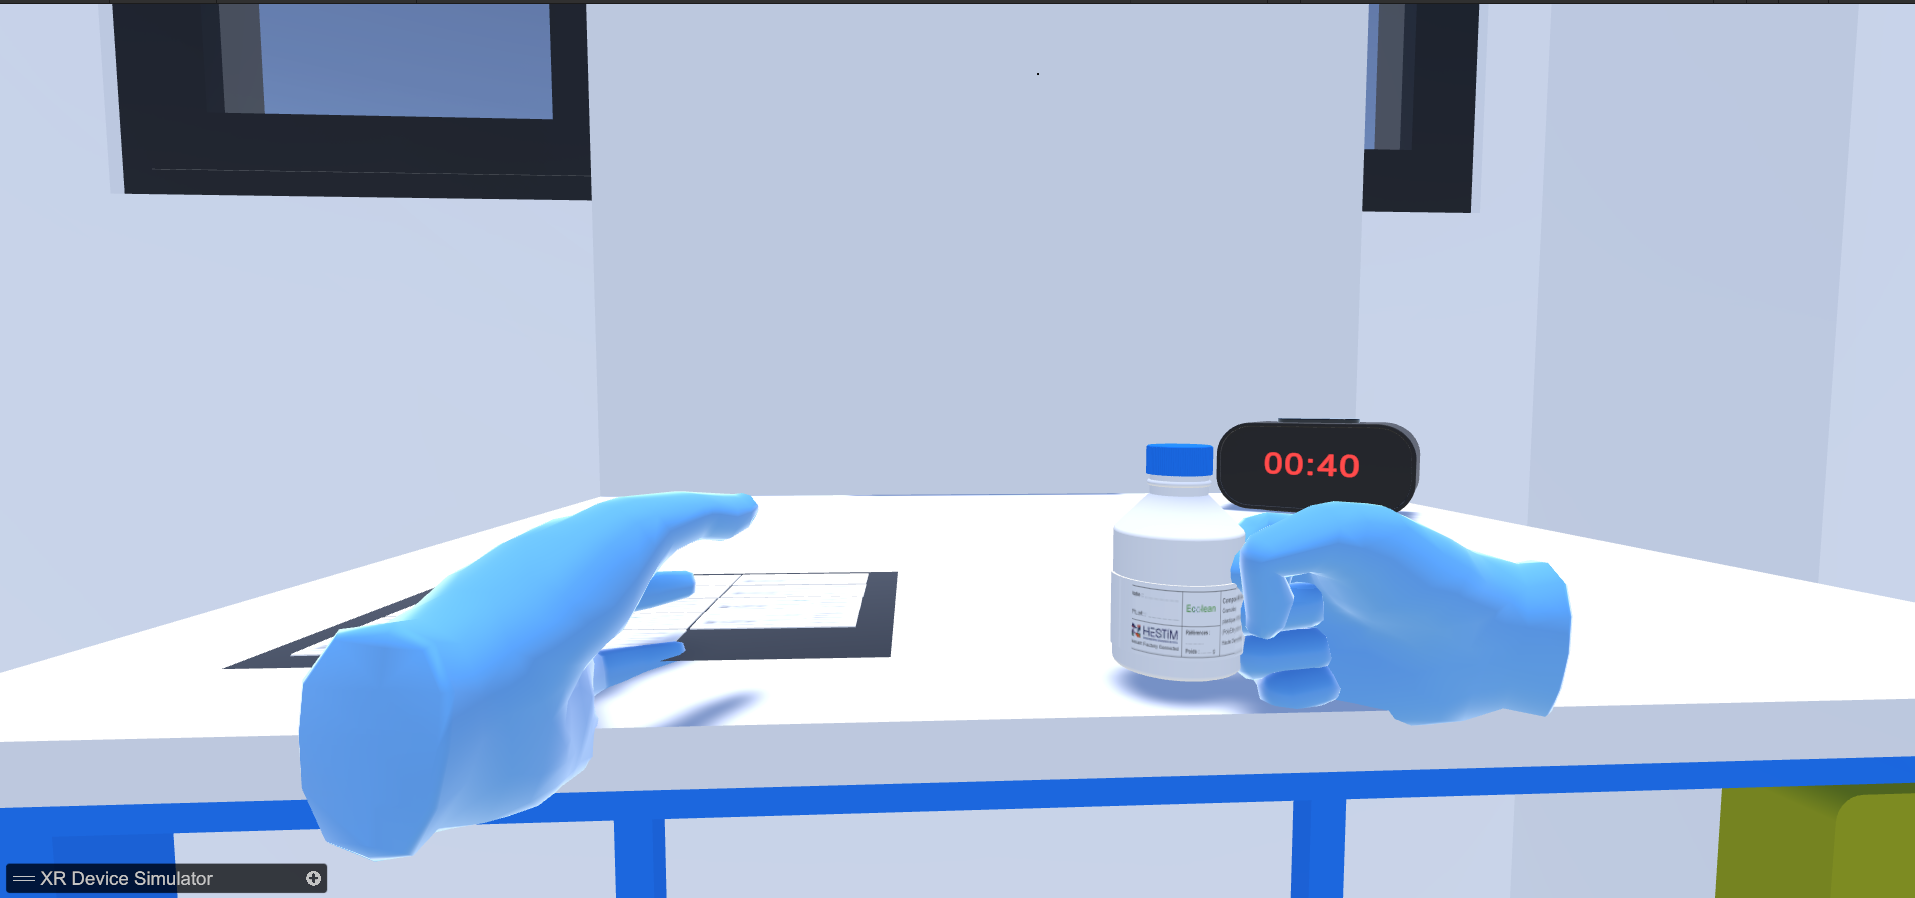
\includegraphics[width=\columnwidth,height=4.1cm,keepaspectratio]{figures/vr_workstation.png}
    \caption{Operator view of the immersive labeling workstation. The virtual hands, bottle, label, timer, and spatial work area form the human-facing layer of the system.}
    \label{fig:workstation}
\end{figure}

\begin{figure*}[t]
    \centering
    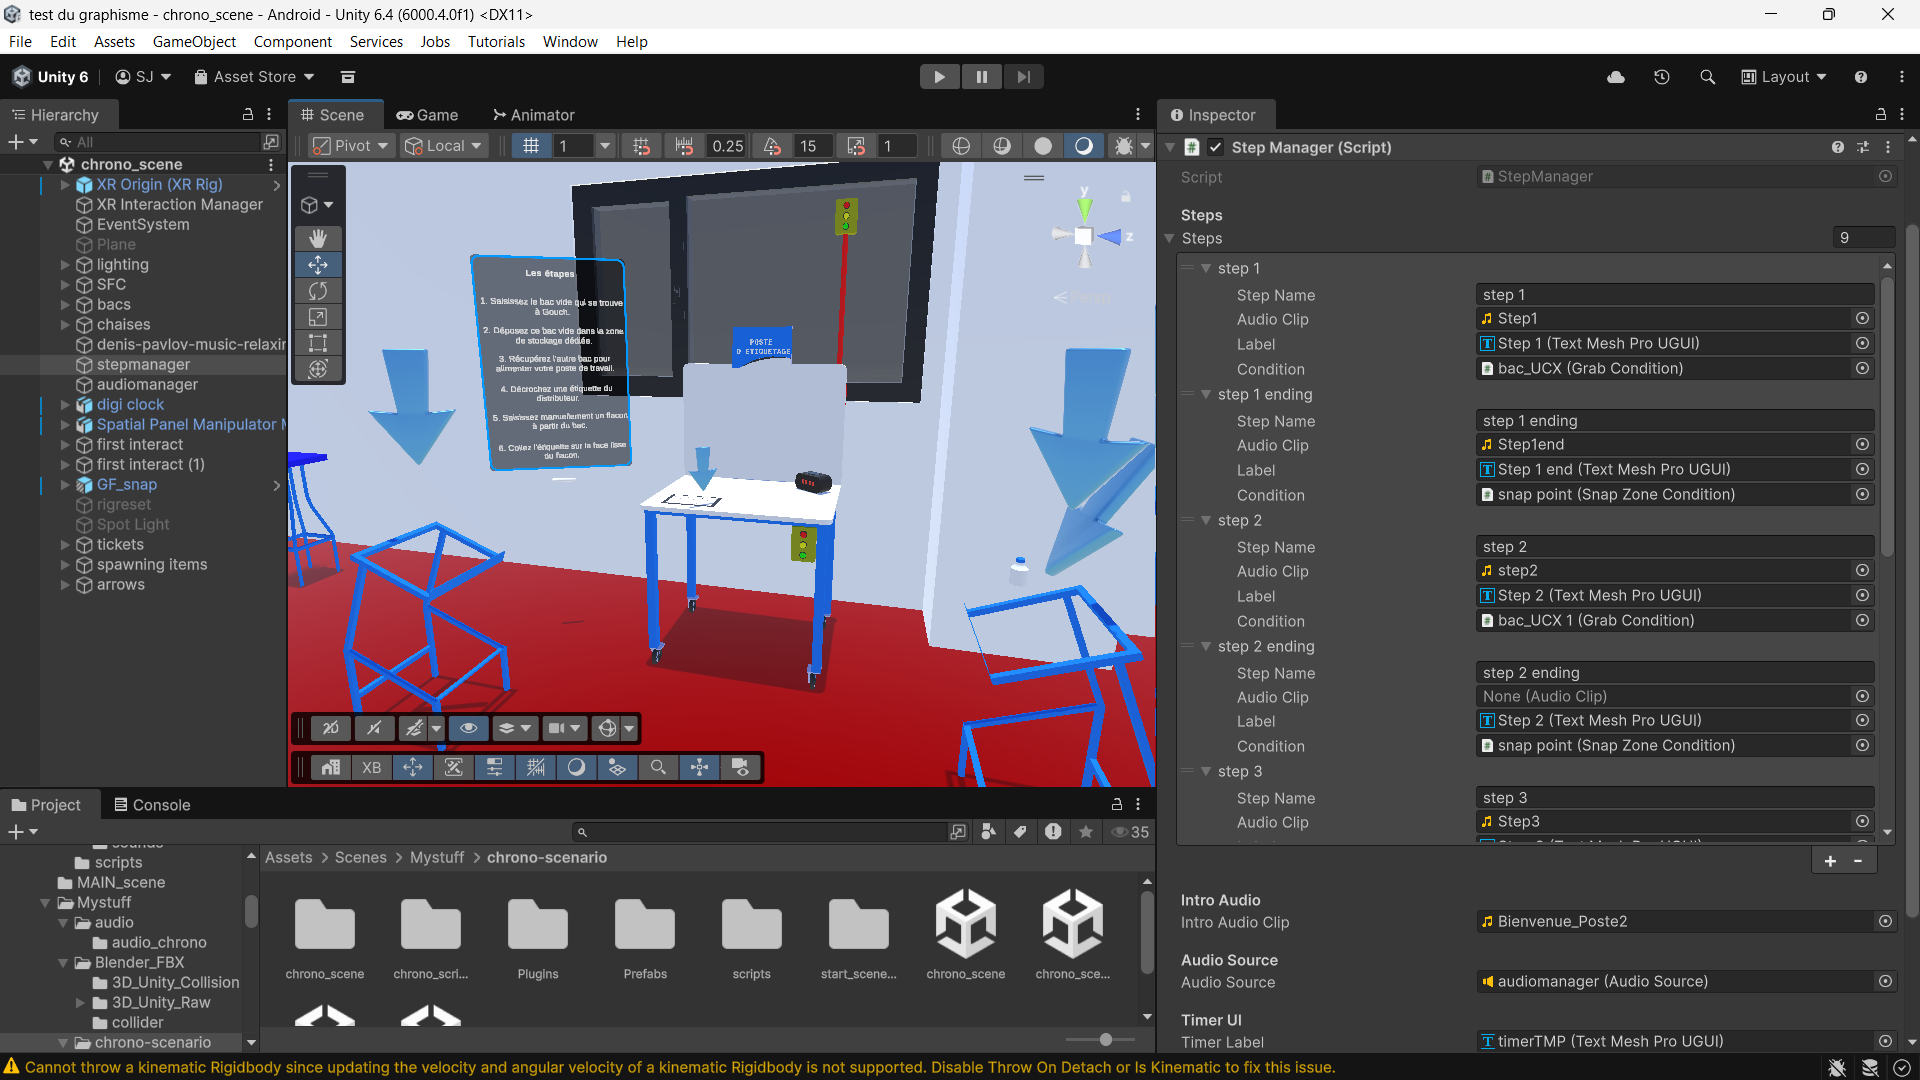
\includegraphics[width=0.88\textwidth,height=7.2cm,keepaspectratio,trim=0 8 0 0,clip]{figures/step_manager.png}
    \caption{Editor-side implementation of the labeling procedure. Each serialized state exposes its instruction, audio cue, interface label, and completion condition, linking the workstation decomposition to the runtime controller.}
    \label{fig:configuration}
\end{figure*}

\subsection{Requirements}

Table~\ref{tab:requirements} links each requirement to an implemented mechanism and functional observation.
The requirements were selected to make the trainer inspectable at runtime. Each one corresponds to a responsibility that must remain explicit in an industrial procedure: preserving task order, rejecting premature actions, separating assistance from validation, protecting participant data, tolerating missing supervision data, and preventing immersive interactions from becoming machine-control commands.

\begin{table}[t]
\caption{Requirement Verification}
\label{tab:requirements}
\centering
\scriptsize
\renewcommand{\arraystretch}{1.12}
\begin{tabular}{@{}p{0.06\columnwidth}p{0.29\columnwidth}p{0.54\columnwidth}@{}}
\toprule
\textbf{ID} & \textbf{Mechanism} & \textbf{Functional evidence}\\
\midrule
R1 & Ordered state controller & Valid execution traversed all nine configured states and closed the session.\\
\midrule
R2 & Rule-based validators & Expected actions advanced the state; unexpected grabs left it active and incremented its counter.\\
\midrule
R3 & Guidance policy & Guided and autonomous runs used identical state identifiers and logging fields.\\
\midrule
R4 & Pseudonymous export & The publication copy removed names, demographics, and exact timestamps.\\
\midrule
R5 & Optional supervision & The labeling scenario executed while the physical-data service was unavailable.\\
\midrule
R6 & Read-only boundary & Inspection found an ESP32-to-Unity data route and no XR-to-actuator route.\\
\bottomrule
\end{tabular}
\end{table}

\FloatBarrier

\section{Platform Architecture}

\subsection{Layered Organization}

Fig.~\ref{fig:architecture} separates two runtime paths. The standalone training path converts XR input into semantic events, evaluates them against the active state, and records aggregate evidence. The optional supervision path transports a physical measurement through a mediation service to a read-only Unity display. No dependency arrow connects supervision availability to procedural execution.

\begin{figure}[t]
\centering
\resizebox{0.94\columnwidth}{!}{%
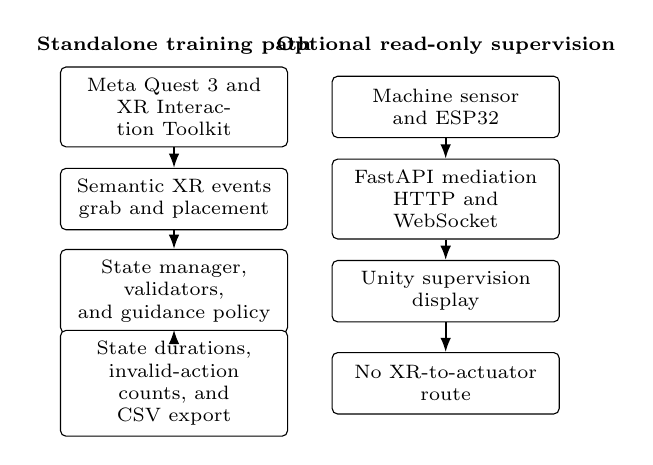
\begin{tikzpicture}[
    box/.style={draw=black, fill=white, text=black, rounded corners=2pt, minimum height=0.78cm, text width=2.65cm, inner ysep=4pt, align=center, font=\scriptsize},
    heading/.style={font=\scriptsize\bfseries, align=center},
    arrow/.style={-{Latex[length=1.8mm]}, semithick}
]
\node[heading] (trainhead) at (0,0) {Standalone training path};
\node[box] (xr) at (0,-0.78) {Meta Quest 3 and\\XR Interaction Toolkit};
\node[box] (events) at (0,-1.95) {Semantic XR events\\grab and placement};
\node[box] (procedure) at (0,-3.12) {State manager, validators,\\and guidance policy};
\node[box] (evidence) at (0,-4.29) {State durations, invalid-action\\counts, and CSV export};

\node[heading] (superhead) at (3.45,0) {Optional read-only supervision};
\node[box] (sensor) at (3.45,-0.78) {Machine sensor\\and ESP32};
\node[box] (api) at (3.45,-1.95) {FastAPI mediation\\HTTP and WebSocket};
\node[box] (display) at (3.45,-3.12) {Unity supervision\\display};
\node[box] (boundary) at (3.45,-4.29) {No XR-to-actuator\\route};

\draw[arrow] (xr) -- (events);
\draw[arrow] (events) -- (procedure);
\draw[arrow] (procedure) -- (evidence);
\draw[arrow] (sensor) -- (api);
\draw[arrow] (api) -- (display);
\draw[arrow] (display) -- (boundary);
\end{tikzpicture}}
\caption{Runtime responsibility boundaries. Training and read-only supervision are separate paths; loss of the optional service does not interrupt procedural execution.}
\label{fig:architecture}
\end{figure}

\subsection{XR Interaction Layer}

The Unity 6 scene uses the XR Interaction Toolkit and contains an XR Origin, an XR Interaction Manager, interactive bottles and bins, snap zones, spatial panels, audio sources, and task-specific animation. Controller or hand interaction is converted into selection and placement events by the XR layer. The procedure controller does not interpret low-level pose data. It receives semantically meaningful events such as ``object grabbed'' or ``object entered target zone.'' This boundary follows the portability goal of OpenXR, which provides a common application interface across conformant XR runtimes \cite{OpenXR}.

Teleportation and turning support movement in the scene, but locomotion does not advance the procedure. State progression occurs only when a registered completion condition is satisfied. Consequently, exploration and accidental contact can be distinguished from task completion.

\subsection{Procedural State Machine}

Let the internal task model be an ordered state set
\begin{equation}
\mathcal{S}=\{s_1,s_2,\ldots,s_n\}, \qquad n=9,
\end{equation}
where a state is represented conceptually as
\begin{equation}
s_i=\langle l_i,a_i,c_i,g_i\rangle.
\end{equation}
Here, $l_i$ is the displayed instruction, $a_i$ is an optional audio clip, $c_i$ is the completion condition, and $g_i$ identifies associated guidance objects. These fields correspond to the serialized configuration visible in Fig.~\ref{fig:configuration}. The state becomes active at time $\tau_i^{a}$ and completes at $\tau_i^{c}$, producing duration $d_i=\tau_i^{c}-\tau_i^{a}$.

Fig.~\ref{fig:state_machine} shows the runtime logic. On activation, the controller updates the instruction panel and cues. A valid interaction completes the state, records its duration, deactivates its cues, and activates the next state. An invalid grab leaves the state unchanged and increments its error counter. The final state closes and exports the session.

\begin{figure}[t]
\centering
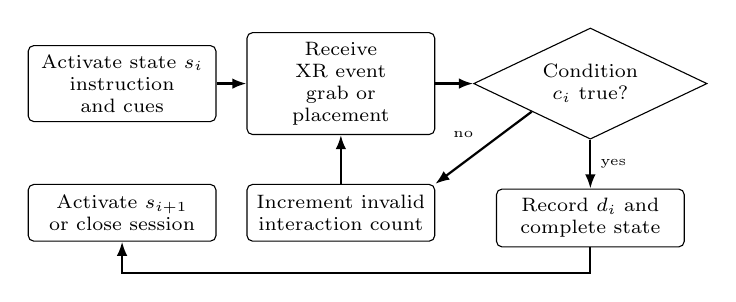
\begin{tikzpicture}[
    state/.style={draw=black, fill=white, text=black, rounded corners=2pt, text width=2.15cm, minimum height=0.72cm, align=center, font=\scriptsize},
    decision/.style={diamond, draw=black, fill=white, text=black, aspect=2.1, align=center, font=\scriptsize},
    data/.style={draw=black, fill=white, text=black, rounded corners=2pt, text width=2.15cm, minimum height=0.72cm, align=center, font=\scriptsize},
    arrow/.style={-{Latex[length=1.8mm]}, thick}
]
\node[state] (activate) {Activate state $s_i$\\instruction and cues};
\node[state, right=0.38cm of activate] (event) {Receive XR event\\grab or placement};
\node[decision, right=0.48cm of event] (valid) {Condition\\$c_i$ true?};
\node[data, below=0.62cm of event] (invalid) {Increment invalid\\interaction count};
\node[data, below=0.62cm of valid] (record) {Record $d_i$ and\\complete state};
\node[state, left=0.38cm of invalid] (next) {Activate $s_{i+1}$\\or close session};
\draw[arrow] (activate) -- (event);
\draw[arrow] (event) -- (valid);
\draw[arrow] (valid) -- node[right,font=\tiny] {yes} (record);
\draw[arrow] (record.south) -- ++(0,-0.32cm) -| (next.south);
\draw[arrow] (valid.south west) -- node[above left,font=\tiny] {no} (invalid.north east);
\draw[arrow] (invalid) -- (event);
\end{tikzpicture}
\caption{State transition and interaction-validation logic. Invalid actions are observable but do not advance the procedure.}
\label{fig:state_machine}
\end{figure}

\subsection{Completion Conditions and Guidance}

Two condition families are used in the labeling implementation. A grab condition verifies that the expected object has been selected during the active state. A snap-zone condition verifies placement in a designated spatial region. The final label-placement condition also triggers the application animation. Keeping the condition as a configurable state field allows different task objects to reuse the same controller logic.

Guidance is implemented as a policy over the state definition. In guided mode, the active instruction, audio clip, and spatial indicators are enabled. In autonomous mode, the procedure and validators remain active while assistance is suppressed. A perturbed mode can introduce scene constraints without changing the logging contract. Thus, guidance changes the available cues while the configured completion rules and evidence fields remain unchanged.

\subsection{Telemetry Pipeline}

When a session starts, the recorder creates a session context and initializes timers and error counters. Each state transition appends its duration. An interaction involving an unexpected object increments the active state's invalid-grab counter. At completion, the recorder exports the structure
\begin{equation}
R=\langle p,t,m,T,\{d_i\}_{1}^{n},\{e_i\}_{1}^{n}\rangle,
\end{equation}
where $p$ is a session identifier, $t$ is the session timestamp, $m$ is the scene or training mode, $T$ is total duration, and $e_i$ is the invalid-interaction count for state $i$.

The runtime CSV contains operational metadata, total duration, nine step-duration fields, and nine invalid-grab-count fields. It is an aggregate session record rather than an immutable event stream: individual invalid actions are counted but not timestamped or identified. The publication copy excludes names, demographic attributes, and exact timestamps, and replaces identity fields with generated session identifiers. The confidential source file remains separate. All participants provided written informed consent.

\section{Digital-Twin-Ready Supervision}

\subsection{Communication Path}

The connected component validates a physical-to-digital path using a temperature measurement from the extrusion-blow-molding machine. An ESP32 sends the value over the local wireless network. FastAPI was selected because one Python service could validate incoming data and expose HTTP and WebSocket interfaces; no comparative framework benchmark was performed. HTTP supports ingestion and snapshot retrieval, while WebSocket pushes updates without application-level polling by the Unity client. Unity therefore depends on the mediation interface rather than the ESP32 message format. The measurement provides line-level supervision and does not alter labeling-state progression. Fig.~\ref{fig:dt_path} documents the implemented HTTP request path and the resulting supervisory view used during integration.

\begin{figure}[H]
\centering
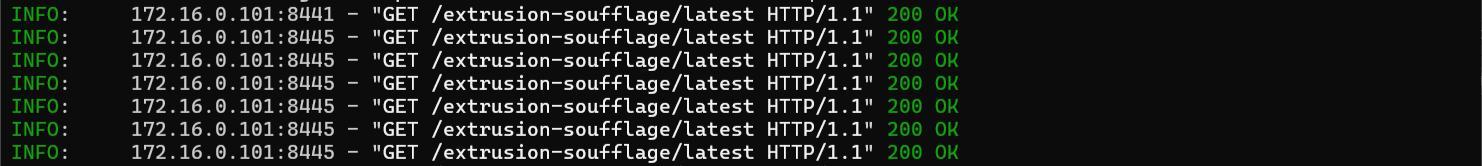
\includegraphics[width=\columnwidth,trim=0 0 250 0,clip]{figures/fastapi_server_runtime.png}\\[-1pt]
{\scriptsize (a) FastAPI request trace}\\[3pt]
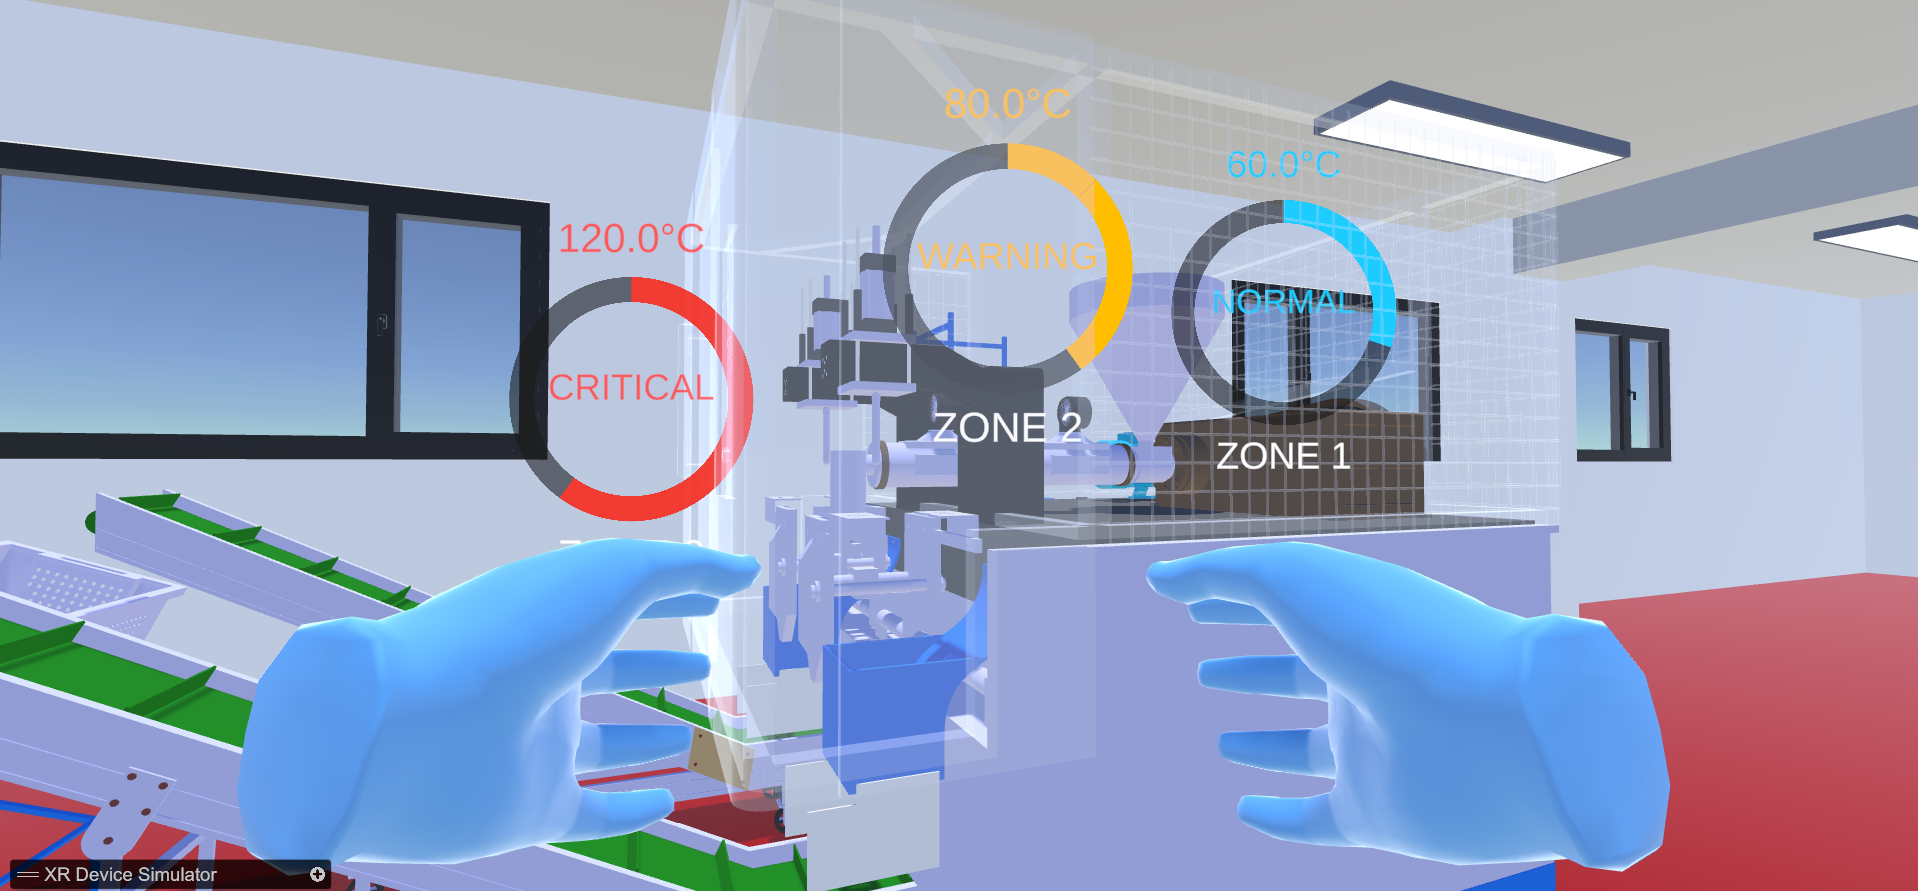
\includegraphics[width=\columnwidth]{figures/unity_temperature_supervision.png}\\[-1pt]
{\scriptsize (b) Unity temperature-supervision view}
\caption{Runtime evidence of the supervision path: (a) the FastAPI service returned HTTP 200 responses to successive snapshot requests; and (b) Unity presented temperature zones in the immersive interface. The screenshots demonstrate integration, not synchronized latency or reliability.}
\label{fig:dt_path}
\end{figure}

\subsection{Scope and Failure Boundary}

This connection is deliberately separated from the labeling trainer. The implemented training scenario operates when the service is unavailable. A production supervision interface would additionally need explicit fresh, stale, and disconnected states; those behaviors were not benchmarked here. The current path is unidirectional and sends no control command to production equipment. It is therefore a read-only supervision baseline rather than a bidirectional operational twin.

The boundary also limits safety risk. FastAPI mediates data formats and communication, while Unity remains a visualization and training client. No path from an XR interaction to a machine actuator is provided.

\begin{figure*}[t]
\centering
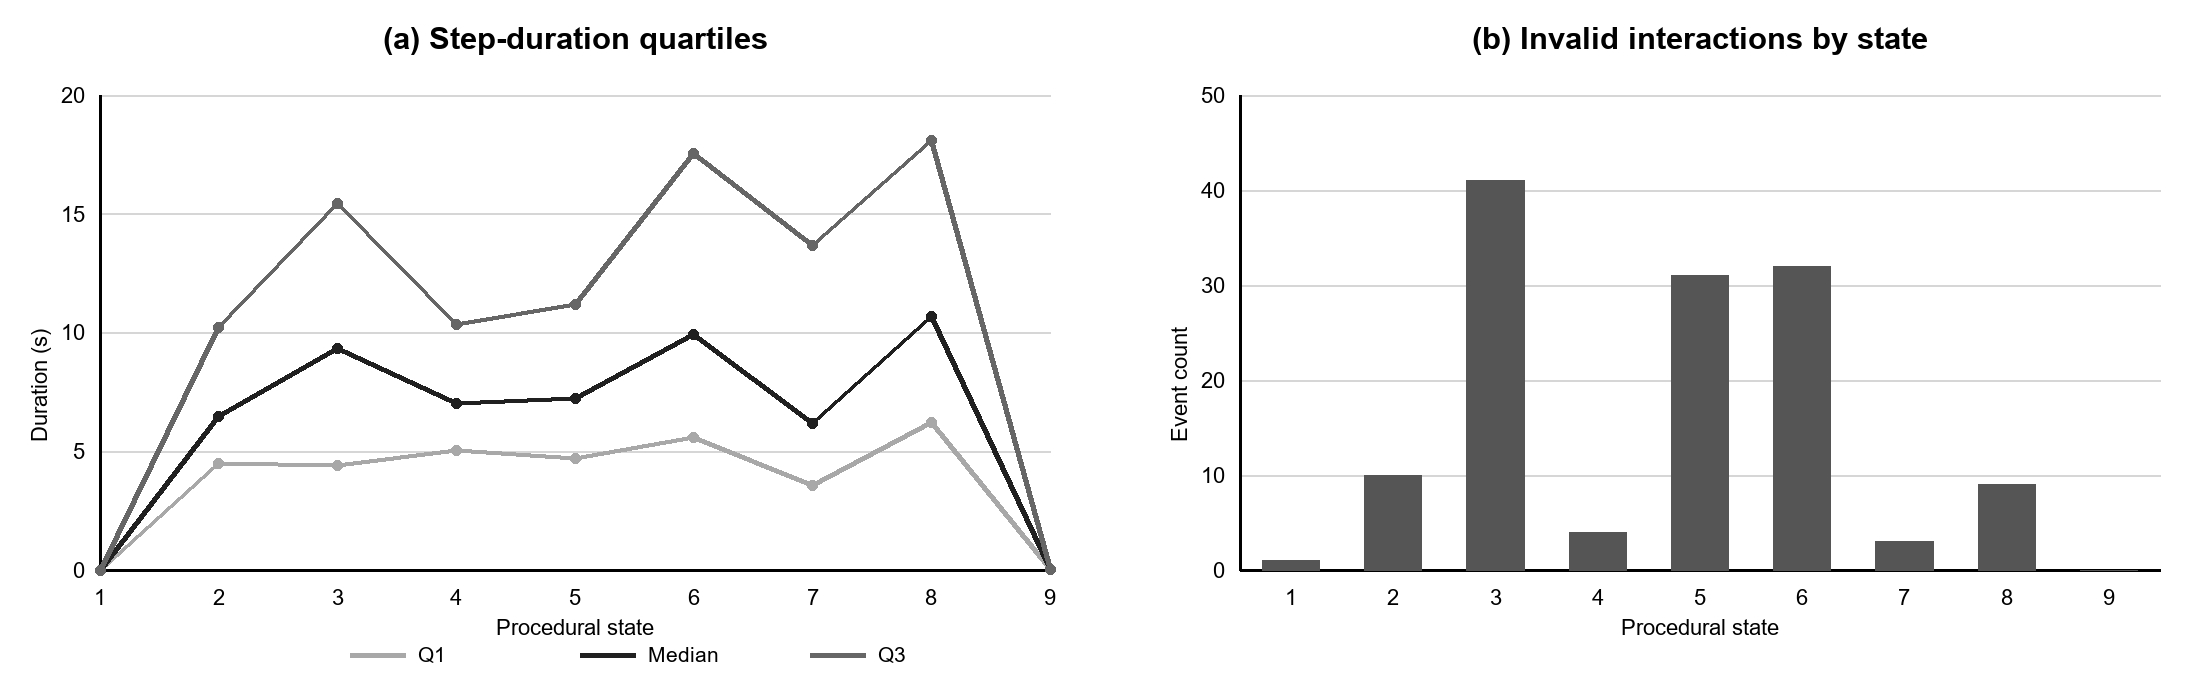
\includegraphics[width=\textwidth]{figures/state_telemetry_results.png}
\caption{State-level telemetry from 36 retained sessions: (a) first quartile, median, and third quartile of duration by procedural state; and (b) invalid-interaction counts by state.}
\label{fig:telemetry_results}
\end{figure*}

\section{Technical Evaluation}

\subsection{Prototype Configuration}

The prototype was developed in Unity 6 with the XR Interaction Toolkit, an XR Origin, and an XR Interaction Manager. It targets a Meta Quest 3 headset. The labeling scene includes interactive bins, bottles, labels, placement zones, world-space instruction panels, arrows, audio guidance, a timer, and a result view. Fig.~\ref{fig:workstation} shows the trainee's workspace, while Fig.~\ref{fig:configuration} shows the editor-side procedure configuration.

The scenario was exercised in guided, autonomous, and perturbed configurations. These modes use the same state identifiers and recorder. Consequently, changing the guidance policy does not require separate logging code or a different data schema.

\subsection{Measured Results}

The source export contained 39 rows because corrected records for one participant had been appended rather than replacing the earlier rows. Processing collapsed exact duplicates and retained the latest timestamp for each participant--condition pair; retained and superseded source-row identifiers were stored for audit. This yielded 36 records from 12 consenting students: seven in Industrial Engineering (GI) and five in Computer Engineering (GIN). All retained records populated the scene identifier, total duration, nine state-duration fields, and nine state-level counters. The counters contained 131 invalid interactions across 31 sessions, showing that rejected actions were represented in the aggregate export.

Recorded session duration ranged from 19.097 to 180.286~s, with a mean of 78.056~s and a median of 71.972~s. The median absolute difference between total duration and summed state durations was below 0.001~s, and 29 of 36 records reconciled within approximately 1~ms. Seven larger residuals ranged from $-0.515$ to $+14.990$~s; these raised the mean absolute difference to 0.986~s. Without explicit session-boundary event timestamps, the residuals cannot be assigned to loading, calibration, or a particular transition. State progression is rule-governed, but exact temporal attribution requires timestamped session-start, state-transition, invalid-action, and session-end events. No hypothesis test, condition comparison, or learning-effect claim is made.

Fig.~\ref{fig:telemetry_results} resolves the same records by procedural state. States 6 and 8 have the largest upper quartiles. Invalid interactions are concentrated in states 3, 5, and 6, which account for 104 of 131 events (79.4\%). The state-specific fields expose where validator counts accumulate, but the aggregate records do not reconstruct individual action sequences. The pattern is not interpreted as evidence of participant learning.

\subsection{Architectural Value}

The demonstration supports three technical observations. The serialized state list exposes sequence and completion rules outside scene callbacks. Validators separate generic XR interaction from task-specific acceptance. Finally, controller transitions and telemetry fields share state identifiers, enabling state-level comparison between configured rules and exported aggregates. Event-level traceability would require the additional timestamps identified above.

\section{Discussion}

\subsection{Scientific and Engineering Implications}

The architecture makes procedural training inspectable at the system level. A scenario can be checked to verify that every state has a completion rule, every invalid action has a defined consequence, and every transition has a corresponding record. The XR rig, recorder, guidance service, and condition types are separated from task-specific scene objects and state sequences.

The communication boundary supports incremental extension because Unity consumes mediated updates rather than communicating directly with embedded hardware. Separating this path from the state manager preserved training availability when the service was absent. This is a functional dependency result, not evidence that the connected display is immune to wireless jitter. Packet loss, update latency, reconnection time, multi-client behavior, headset energy cost, and stale-data presentation were not benchmarked.

\subsection{Human-Centered Implications}

Invalid grabs increment a state-level counter without terminating the session. Guidance can be removed without changing completion rules, and loss of the optional service does not remove access to the trainer. These are human-supportive design choices; the present technical evaluation does not show improved learning, well-being, or autonomy. Trainer-facing records should remain pseudonymous and complement rather than replace instructor judgment.

\subsection{Limitations}

The architecture has been evaluated for one manual workstation, so transfer to maintenance or safety procedures remains unverified. The logger stores aggregate session fields rather than an immutable event stream. Exact XR package, FastAPI, Python, and ESP32 firmware patch versions were not archived, which limits replication. The connected path is unidirectional and was assessed for structural decoupling, not communication performance. Finally, the 36 records demonstrate observability only and do not show improved learning relative to another method.

\section{Conclusion}

The research question was addressed by separating semantic XR events, state-specific validators, guidance, aggregate telemetry, and optional supervision into explicit runtime responsibilities. Functional checks showed that expected actions advance the configured procedure, invalid grabs remain recoverable and counted, guidance can change without changing completion rules, and training can run without the read-only service. Thirty-six retained records demonstrated state-level observability while also revealing the need for timestamped boundary events. The ESP32-FastAPI-Unity path adds physical context but neither controls equipment nor constitutes a validated communication benchmark.

\bibliographystyle{IEEEtran}

\bibliography{wincom_paper}

\end{document}
